\documentclass[twoside,11pt]{article}

\usepackage{paper}
\usepackage{tikz}     
\usepackage{xcolor}
\usepackage{amsmath}
\usetikzlibrary{calc}
\usepackage{graphicx}
\usepackage{subcaption}

\ShortHeadings{
%% short title here
Directional Priors in Manifolds
}{
% last name
Posmik}
\firstpageno{1}

\begin{document}

\title{	Directional Priors in Manifold Learning \\
\vspace{.1in}
PHP2530			
}

\author{ Daniel C. Posmik }

\maketitle
\date{4 }

\section{Introduction} \label{sc:intro}

Manifold learning is dimensionality reduction technique that has proven useful in settings where data are high-dimensional and non-linear. Often, manifold learning algorithms are used when the topological structure of the data are to be preserved in a statistical learning task\footnote{For an introduction, see \citet{Meila2023}}. Within the manifold learning framework, data are assumed to live on a lower dimensional manifold and are corrupted by high-dimensional noise. We say that $D$-dimensional data can be embedded in $d$-dimensional manifold where $d \leq D$ but generally $d \ll D$ .  

\begin{figure}
  \begin{center}
    \begin{tikzpicture}[scale=0.85]
      % Define styles
      \tikzset{
        manifold/.style={blue, thick, fill=blue!10},
        noise/.style={gray, thick},
        observed/.style={blue, thick, fill=blue!10, opacity=0.7},
        arrow/.style={->, >=stealth, thick},
        label/.style={font=\normalfont\normalsize}
      }
      % Low-dimensional manifold (left)
      \begin{scope}[xshift=-5cm]
        \draw[manifold] plot[smooth, tension=0.8] coordinates {(-1.5,0) (-0.5,1) (1,1.2) (1.5,0) (1,-1) (-0.5,-1) (-1.5,0)};
        
        % Draw some points on the manifold
        \node[circle, draw, inner sep=1pt, fill=blue!50] at (-0.7,0.3) {$f$};
        \node[circle, draw, inner sep=1pt, fill=blue!50] at (0.8,0.5) {$f$};
        \node[circle, draw, inner sep=1pt, fill=blue!50] at (0.2,-0.6) {$f$};
      \end{scope}
      % High-dimensional noise (center)
      \begin{scope}
        % Draw noise as radial lines from center point
        \fill (0,0) circle (0.1);
        \foreach \i in {0,10,...,350} {
          \draw[noise] (0,0) -- (\i:1.2+0.3*rnd);
        }
      \end{scope}
      % Observed data (right)
      \begin{scope}[xshift=5cm]
        % First draw the noise pattern
        \fill (0,0) circle (0.1);
        \foreach \i in {0,10,...,350} {
          \draw[noise] (0,0) -- (\i:1.2+0.3*rnd);
        }
        
        % Then overlay the manifold with transparency
        \draw[observed] plot[smooth, tension=0.8] coordinates {(-1.5,0) (-0.5,1) (1,1.2) (1.5,0) (1,-1) (-0.5,-1) (-1.5,0)};
        
        % Draw some points on the manifold
        \node[circle, draw, inner sep=1pt, fill=blue!50, opacity=0.7] at (-0.7,0.3) {$f$};
        \node[circle, draw, inner sep=1pt, fill=blue!50, opacity=0.7] at (0.8,0.5) {$f$};
        \node[circle, draw, inner sep=1pt, fill=blue!50, opacity=0.7] at (0.2,-0.6) {$f$};
      \end{scope}
      % Draw the operation symbols
      \node at (-2.5,0) {$+$};
      \draw[arrow] (2,0.5) -- (3,0.5);
      \draw[arrow] (3,-0.5) -- (2,-0.5);
      % Draw the curved arrows for parametrization and embedding
      \draw[arrow, green!50!black, thick] (-4,2.5) to[bend left=30] node[above, font=\normalfont\normalsize] {Parameterization} (4,2.5);
      \draw[arrow, orange, thick] (4,-2.5) to[bend left=30] node[below, font=\normalfont\normalsize] {Embedding} (-4,-2.5);
      % Labels with consistent position and size
      \node[label, text width=3cm, align=center] at (-5,-2) {Low-dimensional manifold};
      \node[label, text width=3cm, align=center] at (0,-2) {High-dimensional noise};
      \node[label, text width=3cm, align=center] at (5,-2) {Observed data};
    \end{tikzpicture}
  \end{center}
  \caption{Manifold Learning: Parameterization vs. Embedding}\label{fig:manifolds}
\end{figure}

Within the principal manifolds framework \citep{Meng2021} -- a replicable and flexible framework for manifold learning -- the process of fitting a manifold to our data contains multiple steps. The key idea is that we fit a $d$-dimensional manifold to our $D$-dimensional by minimizing the sum of squares between our data and the proposed manifold. An important extension to linear dimensionality reduction, i.e. the principal components algorithm (PCA), is that we allow our proposed manifold to preserve underlying topological structure of our data. In a way, manifold learning reduces the dimensionality of data with an explicit focus on the topology of it. We note that -- although certainly intuitive -- this topological structure is not only limited to spatial abstraction, but may be extended to arbitrary dimensions of interest. This framework was pioneered as an extension to the PCA algorithm with curves (\citet{HastieStuetzle1989}, \citet{Tibshirani1992}) and has since found a myriad of applications in higher-dimensional extensions. 

We now propose a method for incorporating prior distributional information into the principal manifolds framework. 

\section{Background}

Consider a setting where we have fit a manifold $\mathcal{M}_d$ to our $D$-dimensional data by means of minimizing the orthogonal distance between the data and the manifold. We consider this manifold fixed and will not touch on the fitting procedure itself. Given $\mathcal{M}_d$, for each data point, i.e. the row vector $[x_{11} \cdots x_{1D}]^T$, we can now define the point on $\mathcal{M}_d$, say $f\left(\left[x_{11} \cdots x_{1D}\right]^T\right)$. This point minimizes the distance between $x_i$ and $f(x_i)$. We want to stress again that this procedure does not mean we are fitting the manifold to the data, we are simply retrieving the distance-minimizing projection point. We write 

$$
\text{arg~min}_{f \in \mathcal{F}} \|x^* - f(x^*)\|_2
$$

where we consider each projection function $f$ to be a member of an arbitrary function space $\mathcal{F}$. We define the distance metric as the $L^2$ distance. 

If there exists only one projection point $f(x_i)$ for every $x_i$, every $f \in \mathcal{F}$ is one-to-one and onto ("bijective") mapping. We find it interesting to highlight that the projection functions in the PCA algorithm are inherently bijective, and for inferential purposes, this is a property that is often taken for granted\footnote{This is because a principal axes is a straight line, i.e. neither convex or concave. Although a point's distance to its projection may be co-minimal across $\leq 2$ dimensions, it only has one $f(x_i)$ in one principal axis.}. In a manifold learning framework, this is no longer the case. Albeit highly interesting, due to the limited scope of this paper, we shall treat this scenario as an edge case, reserving rigorous treatment for the blissful times that follow the author's qualifying exam. 

Now, given the data $[\{x_i\}_{i=1}^n, \{f(x_i)\}_{i=1}^n]$, we can reparameterize our space into polar coordinates to obtain a vector representation of the collection $f \in \mathcal{F}$. Converting a Cartesian parameterization in space with $D$ dimensions into polar coordinates yields the $d$-dimensional vector $[r_i^*; \theta_{i, 1}, \cdots, \theta_{i, D-1}]$, i.e. one radius $r_i^*$ and a set of $D-1$ angles suffice to characterize each point $x_i$'s location in space. 

Recognize that the parameter $r^*$ is not random. This is because it is simply the result from our previous projection distance-minimizing procedure. Usually, polar parameterizations assume that all angles and radii are centered at the origin. Luckily, simple vector addition and subtraction readily generalizes our parameterizations in space. For instance, to obtain the vector from the point $x_i$ and $f(x_i)$, we simply subtract $f(x_i) - x_i$. It is important that the issue of defining the origin is explicitly clarified when dealing with directional information. For simplicity, we will henceforth consider data centered at the origin.

\begin{figure}
  \begin{center}
    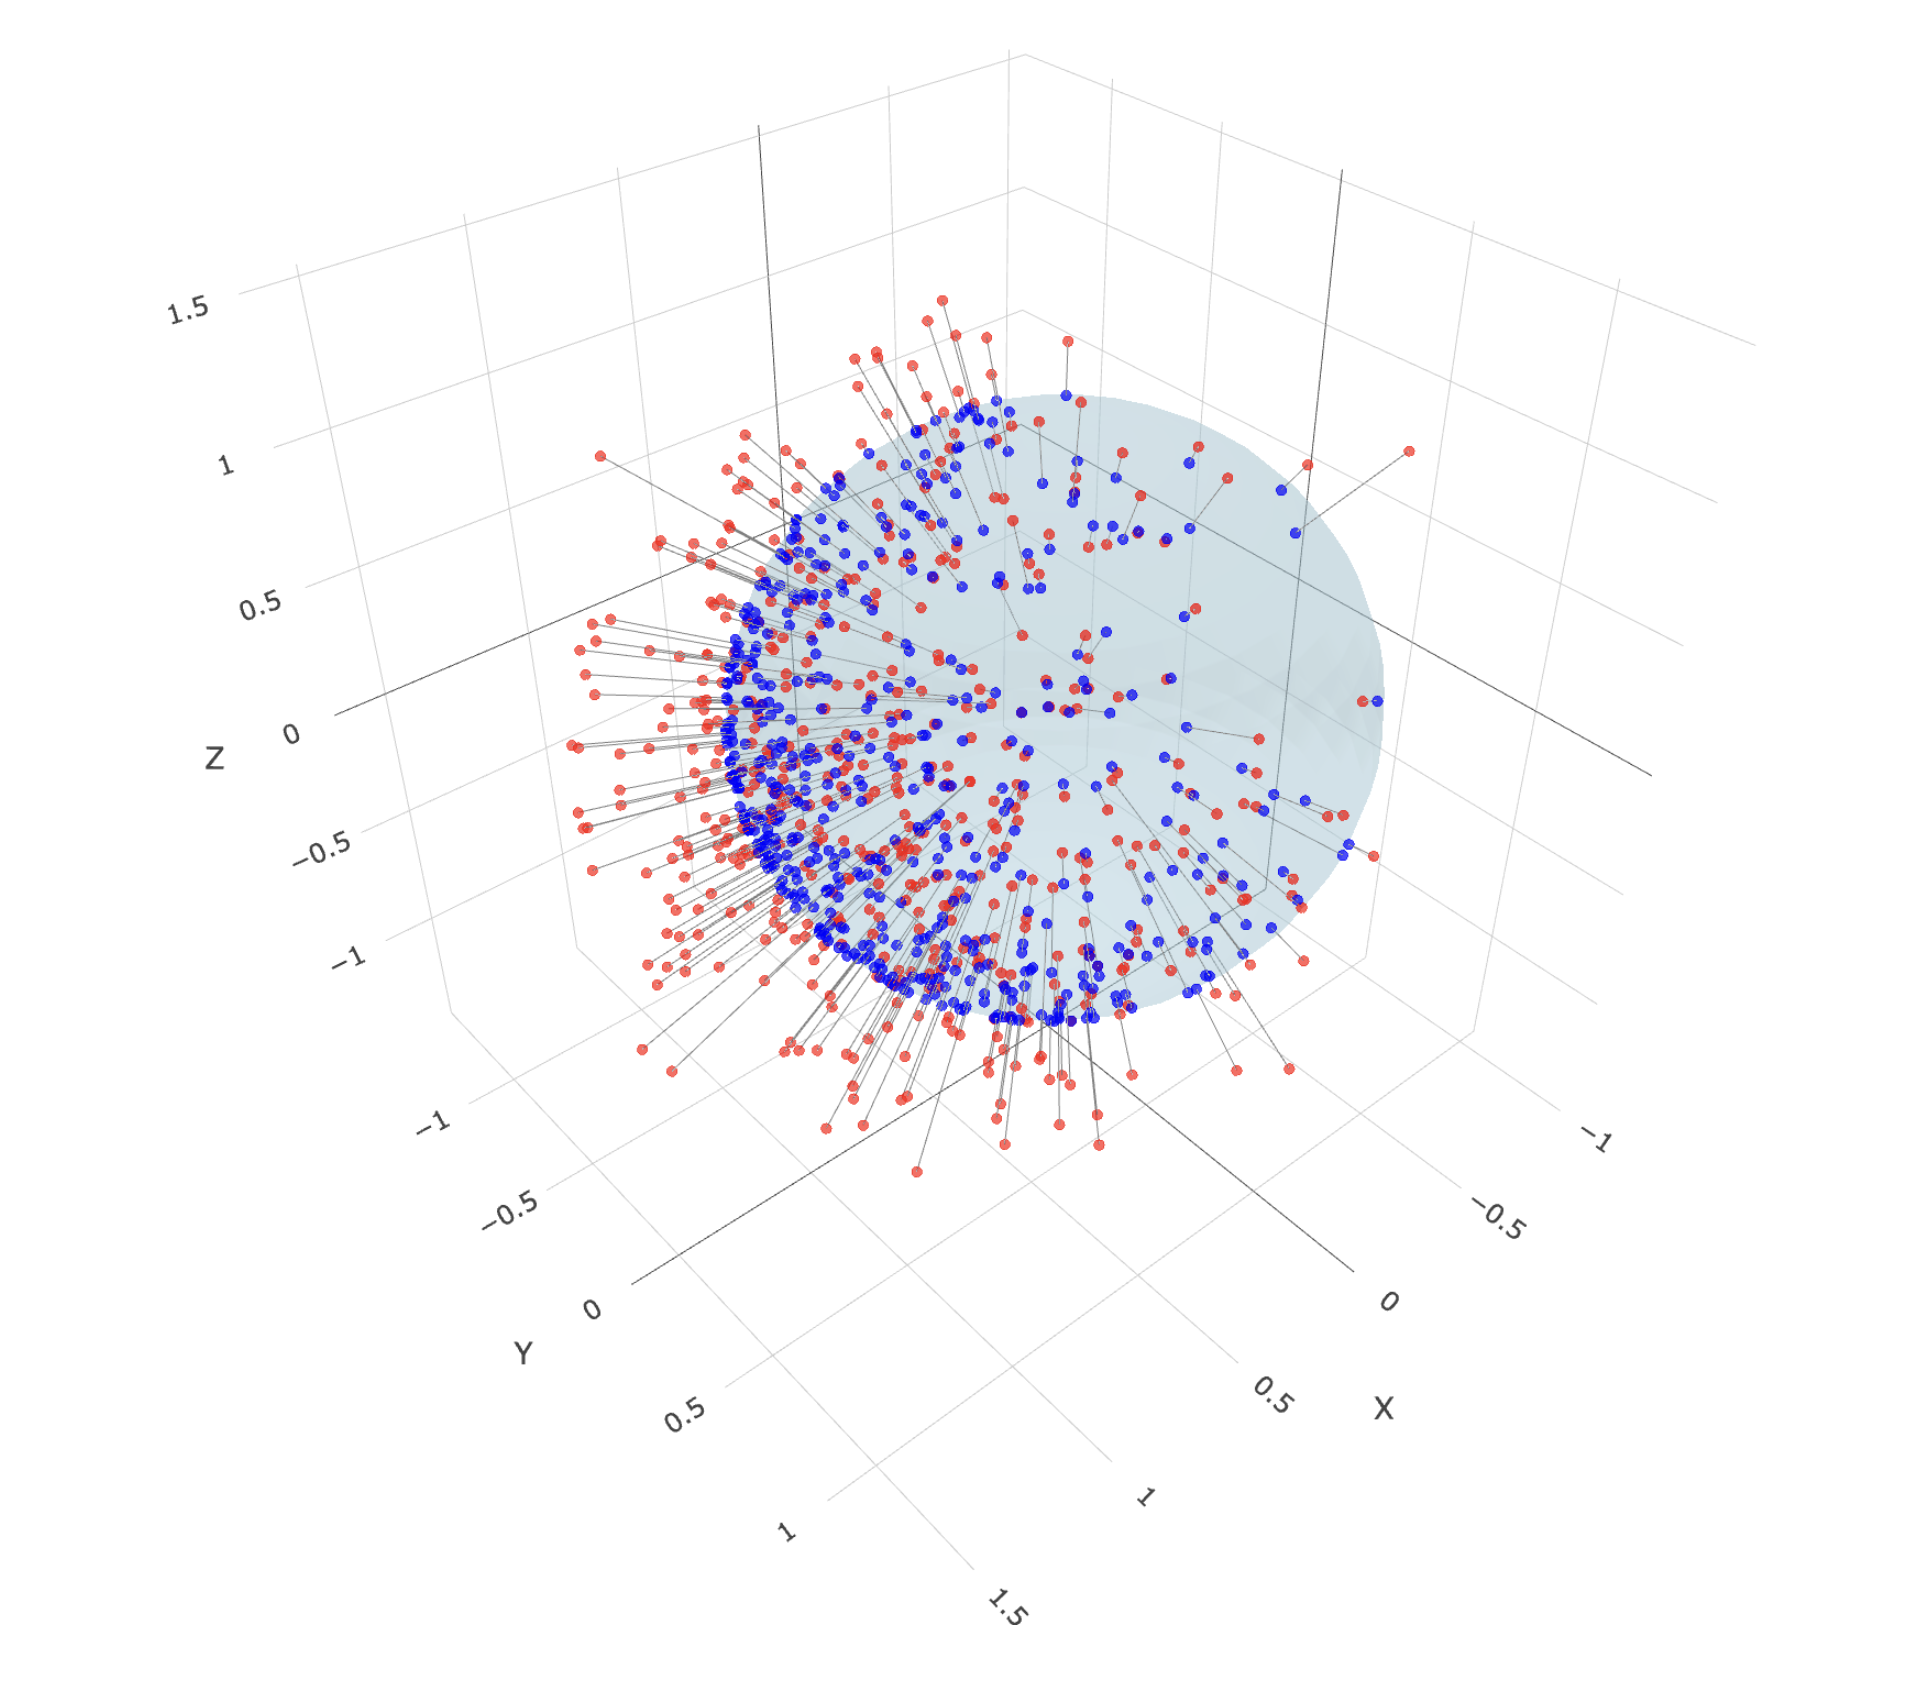
\includegraphics[width=0.75\textwidth]{../fig/data-with-noise.png}
  \end{center}
  \caption{Noisy data projected on $\mathcal{M}_3$; the unit sphere in $\mathbb{R}^3$}\label{fig:data-with-noise}
\end{figure}


\section{Directional Priors}

In contrast to the radii, the $\{D-1\}$-dimensional vector of angles, $\boldsymbol{\theta_i} := [\theta_{i, 1}, \cdots, \theta_{i, D-1}]^T$ is random. In simple terms, $\{r_i, \boldsymbol{\theta}_i\}$ is what parameterizes the realized sample $\boldsymbol{X_i} = x_i$ in space. If we draw multiple samples, the random sampling variation in $\mathbf{\theta}_i$ is what captures the randomness. In biomedical applications, such as cancer medicine, we may have reliable prior information (i.e. from previous trials or expert knowledge) on directional trends of malignant growths. Within a Bayesian framework, using our data to update these prior directional information offers a principled, probabilistic solution to complex inference problems in settings where directionality is a key piece of information.   

Before we formulate our approach formally, we briefly introduce directional statistics. When we reparameterized our data from Cartesian coordinates into polar coordinates, we did not address the underlying probabilistic transformations. For example, when encoding uncertainty in a spherical setting, it may be naive to parameterize a normal density with support on $\mathbb{R}^1$ since angles are defined in the interval $[0, 2\pi]$. Directional statistics offer well-defined spherical reparameterizations of distributions, such as the normal. Instead of defining a mean vector in $\mathbb{R}^1$, we can define a mean directional vector contained in $[0, 2\pi]$. To account for the infinite support, the wrapped normal is defined on a support of $k\text{mod}(2\pi)$. Henceforth, unless stated otherwise, we will deal with the spherical parameterizations of densities to account for the spherical parameterization of our problem. 

\subsection{Motivating Example: 3D Sphere}

We begin our discussion with an example of a 3D sphere. As discussed, this means that we have some simulated noisy data $\{x_i\}_{i=1}^n$ in 3D space. The noisy data is projected on the manifold of choice, i.e. the unit sphere. This yields the data $\{f(x_i)\}_{i=1}^n$. These data are parameterized in a polar coordinate system with $\{r_i, \mathbf{\theta}_i\}$, where the (non-random) radius $\vec{r_i}$ is the vector from the origin to $f(x_i)$. Since we are in 3D space, we have two angles. One angle, $\{\mathbf{\theta}\}_{i=1}^n$, which parameterizes the angle from the origin on the XY-plane. The angle $\{\mathbf{\phi}\}_{i=1}^n$ is the angle between the XY-plane and the point $f(x_i)$. 

\begin{figure}
  \begin{center}
    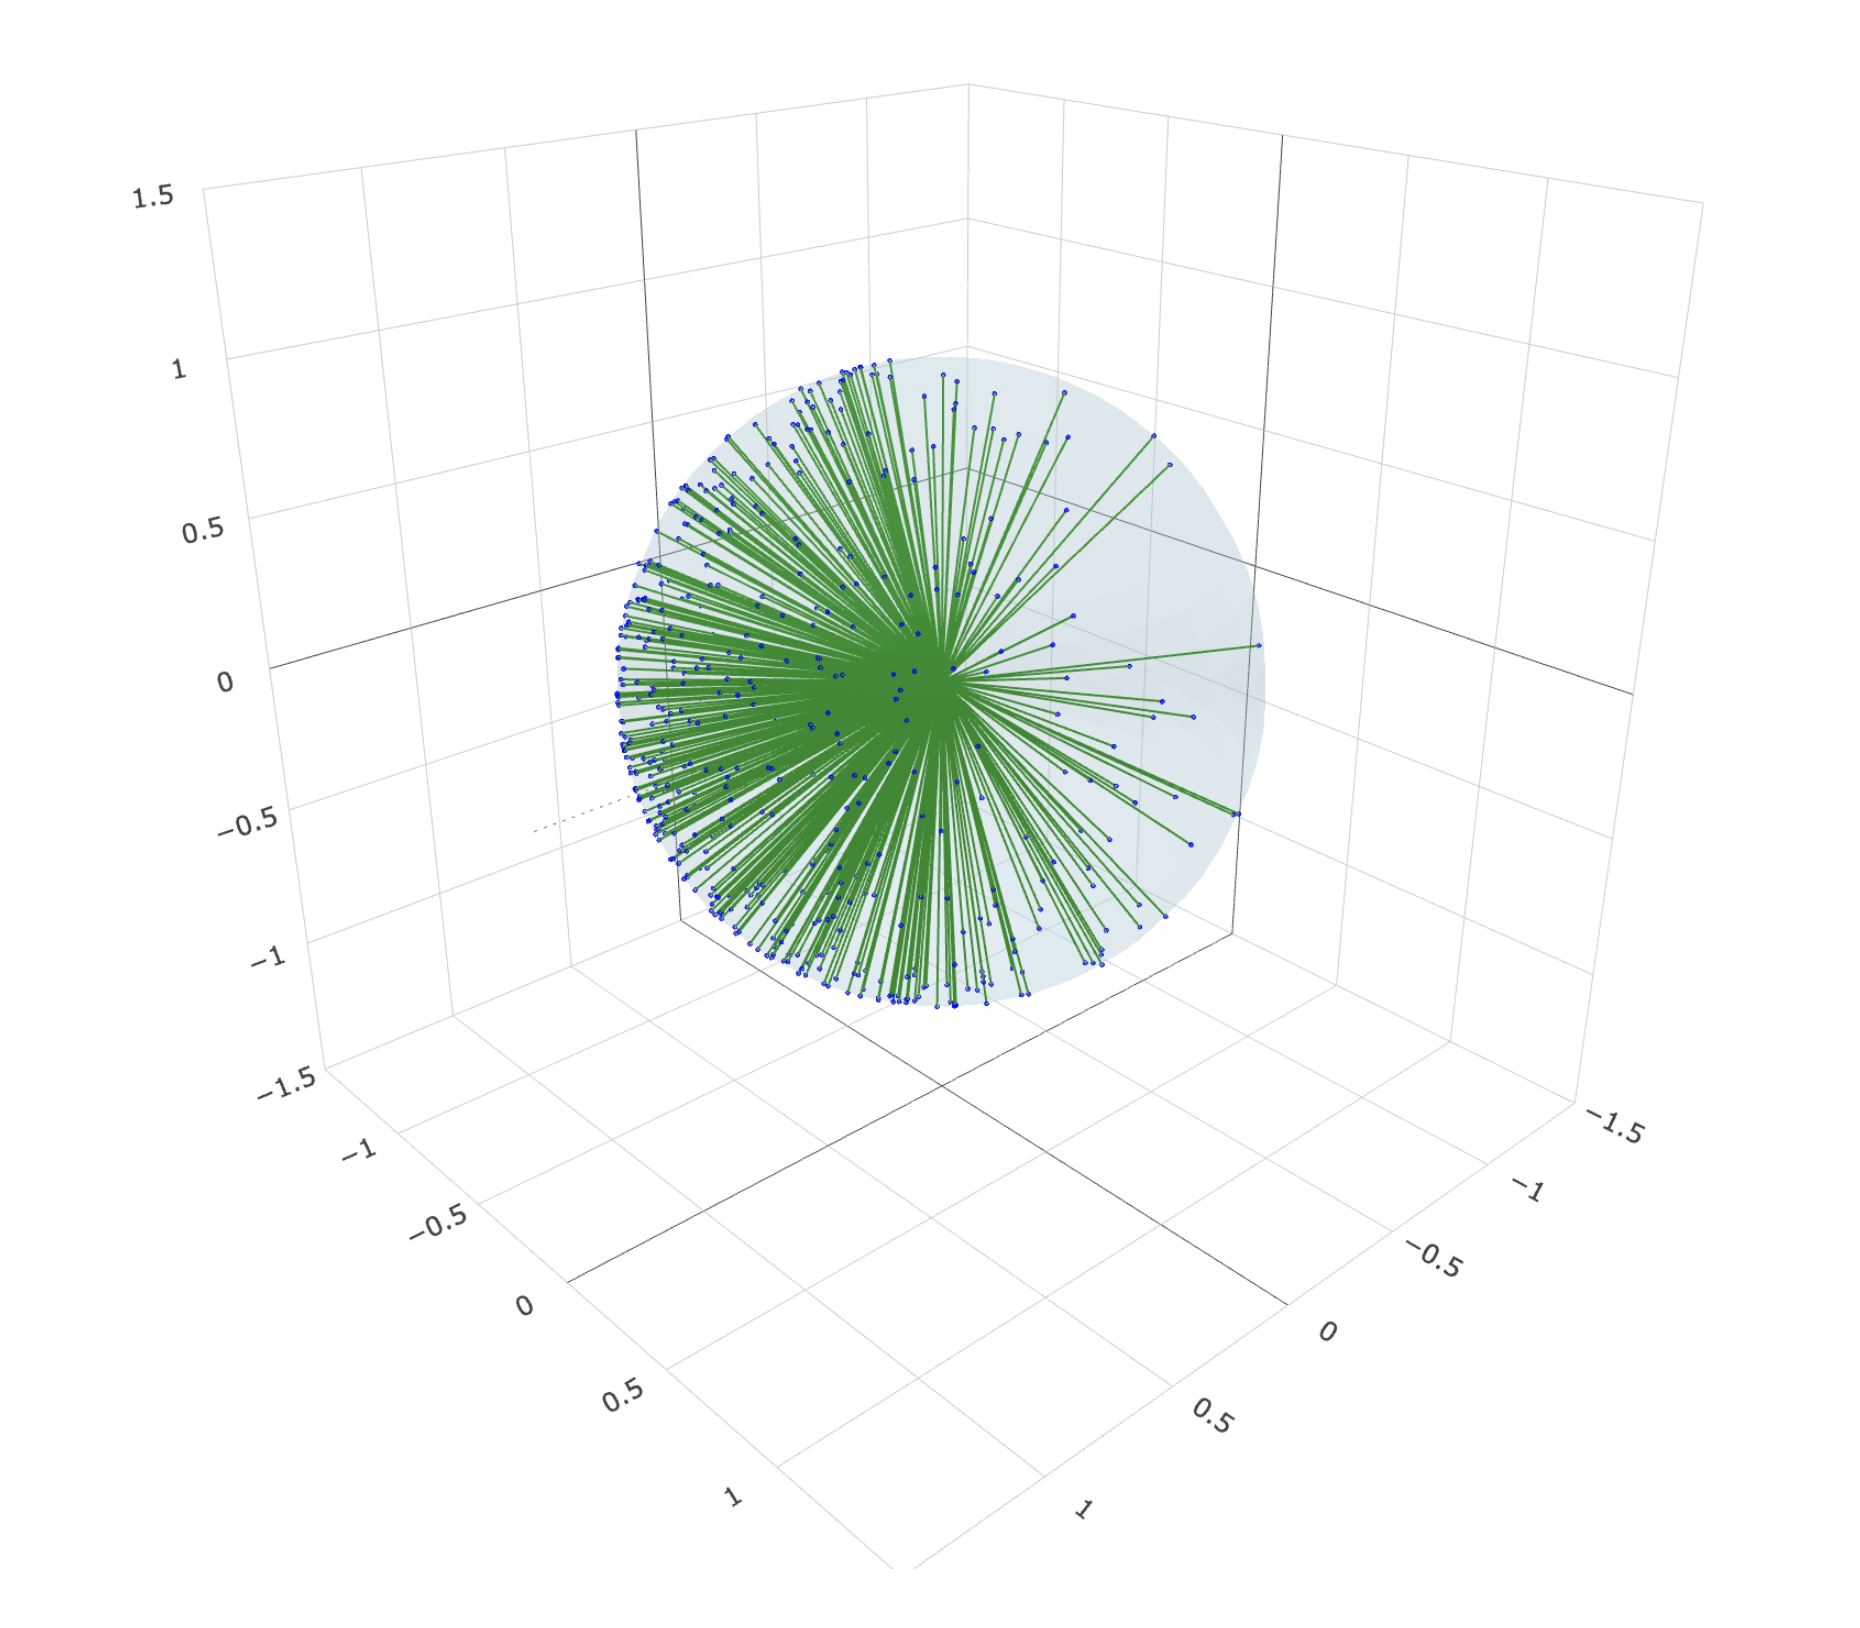
\includegraphics[width=0.75\textwidth]{../fig/projections-from-origin.png}
  \end{center}
  \caption{Polar parameterization with $\{r_i, \theta_i, \phi_i\}$ of projected data}\label{fig:projections-from-origin}
\end{figure}

\subsection{Formulating Directional Priors}

Formulating a directional prior is not trivial. For one, it is important to set a reference point for both the directional prior and the angles. It is important that all angles are measured from the same reference point. For simplicity, we choose the origin. Now, choosing a directional prior in some direction $\mu \in [0, \pi]$ allows\footnote{Note that we choose prior means are only meaningful in $[0, \pi]$ This is because for any prior mean greater than $\pi$, we would consider the closer angle in the opposite direction.} us to incorporate information on where the projected points should be concentrated on the manifold. We only posit a prior on the random set $\{\theta_i\}_{i=1}^n$, expressing some prior distributional belief on the concentrations of points in the XY-plane. In this example, we consider the angles $\{\phi_i\}_{i=1}^n$ to be fixed, making our example univariate. An extension to the multivariate case would be straightforward by using the multivariate analogoues of our likelihood and prior distribution functions. 

Our posterior distribution on the random vector $\theta$ can be expressed as follows. 

\[
\begin{aligned}
  f_{\theta | \mu} (\theta | \mu) 
  &\propto \left\{ \prod_{i=1}^n f_{\theta_i | \mu}(\theta_i | \mu) \right\} \cdot f_{\mu}(\mu) \\ 
  &\propto \mathcal{L}(\theta | \mu) \cdot f_{\mu}(\mu) 
\end{aligned}
\]

where $\boldsymbol{\mu}$ is our mean vector that we posit a prior on, i.e. $\mu \sim f_{\mu}(\mu)$. To form our likelihood, we rely on the wrapped ("spherical") normal distribution. The density of a wrapped normal is given by 

$$
f(\theta|\mu,\sigma^2) = 
\frac{1}{2\pi\sigma^2} \sum_{k=-\infty}^{\infty} \exp\left(-\frac{(\theta-\mu+2\pi k)^2}{2\sigma^2}\right)
$$

with the infinite support reflected in the $\mathit{mod}(k)$ argument. Integrating over $2\pi$ is equivalent to integrating over $\mathbb{R}$ in the canonical parameterization. Now, a disadvantage of using the above form is the infinite series. Deriving moments is not straightforward and requires (inverse) Fourier transforms. Thus, we will use the von Mises distribution, an analogue to the spherical normal that is easier to handle. The density of a von Mises distribution is given by 

$$
f(\theta|\mu,\kappa) = \frac{e^{\kappa \cos(\theta-\mu)}}{2\pi I_0(\kappa)}
$$

where $\theta$ is the angle, $\mu$ is the mean direction (location parameter), $\kappa \geq 0$ is the concentration parameter, and $I_0(\kappa)$ is the modified Bessel function of the first kind of order 0. The von Mises distribution is also known as the circular normal distribution and is the circular analog to the normal distribution. As $\kappa$ increases, the distribution becomes more concentrated around the mean direction $\mu$. When $\kappa = 0$, the distribution reduces to the uniform distribution on the circle. Although we will not dive further into this, the von Mises distribution scales nicely for $p$-dimensional hyperspheres in $\mathbb{R}^p$, making the family of von Mises distributions an attractive and flexible candidate for learning tasks in spherical settings. 

\subsection{Variance Encodes Curvature}

In the above parameterization, it is natural to ask how to define the variance in terms of the concentration parameter $\kappa$. Choosing the variance term naively, e.g., a constant, would of course be possible, but would negate the benefits that manifold-learning gives us as a dimensionality reduction technique which preserves local toplogical structure. Thus, we are interested in a principled manner of choosing the variance term that encodes the (dis-)similarity of the topological structure. Intuitively, if we have a directional prior on a region with little topological variation, we may be willing to update our projection more liberally. However, suppose that even a small change in the projection angle moves our data point into an area that is very different from our original projection. In that case, we not be as willing to update our projection. 

In manifolds that spherically parameterized, using the inverse absolute Gaussian curvature is a sensible choice to encoding variance. Interestingly, there is an intuitive connection to the score test in likelihood-based inference, which uses the slope at restricted MLE estimates as a measure of closeness/ similarity. Thus, not only does this solution make intuitive topological sense, it has a strong analogue in well-established likelihood-based methods.  

The Gaussian curvature of a surface can be defined as the product of the principal curvatures:

$$K = k_1 \cdot k_2$$

where $k_1$ and $k_2$ are the principal curvatures at a point on the surface. For a sphere of radius $R$, we can deduce its Gaussian curvature by considering any point on a sphere of radius $R$. At this point, we can find two perpendicular directions that correspond to the principal curvatures. Due to the perfect symmetry of a sphere, the curvature is the same in all directions at any given point. For a sphere, both principal curvatures are equal to $\frac{1}{R}$ (the reciprocal of the radius). Therefore, for our example, the Gaussian curvature is:

$$K = k_1 \cdot k_2 = \frac{1}{R} \cdot \frac{1}{R} = \frac{1}{R^2}$$

For a unit sphere (where $R = 1$), the Gaussian curvature\footnote{This constant Gaussian curvature of 1 is an intrinsic property of the unit sphere and is related to the fact that the total curvature integrated over the entire sphere equals $4\pi$ (by the Gauss-Bonnet theorem)} is $K = \frac{1}{1^2} = 1$. 

\begin{figure}
  \begin{center}
    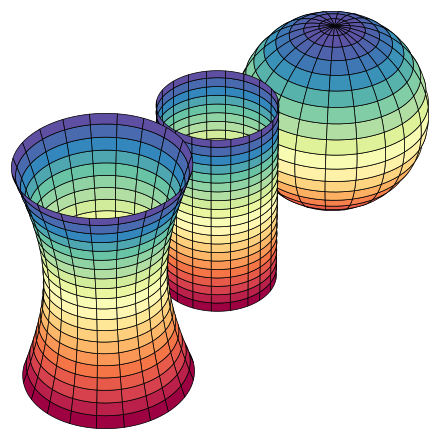
\includegraphics[width=0.5\textwidth]{../fig/gaussian-curvature.png}
  \end{center}
  \caption{From left to right: a surface of negative Gaussian curvature (hyperboloid), a surface of zero Gaussian curvature (cylinder), and a surface of positive Gaussian curvature (sphere).}\label{fig:gaussian-curvature}
\end{figure}

\subsection{Conjugacy}

A key advantage of using the von Mises distribution are conjugacy results. We lean on the work of \citet{mardia1976}. A von Mises prior distribution with mean direction $\mu$ and concentration parameter $\kappa$ (scaled by $c$) is conjugate to the likelihood. After observing angles $\theta_1,\ldots,\theta_n$, the posterior distribution is proportional to the following expression \citep{mardia1976}:

\[
  f(\mu_i, \mu^* | \{\theta_i\}_{i=1}^n) \propto \text{exp}(\kappa \cdot \sum_{i=1}^n \text{cos}(\theta_i - \mu_i) +\kappa^* \cdot \sum_{i=1}^n \text{cos}(\mu_i - \mu^*))  
\]

where the angles $\{\theta_i\}_{i=1}^n \sim \mathcal{VM}(\mu_i, \kappa)$ and the prior on $\mu_i$ is $\mu_i \sim \mathcal{VM}(\mu^*, \kappa^*).$\footnote{$\mathcal{VM}(\cdot, \cdot)$ denotes the von Mises distribution} In our case, we generated the data with $\mu_i = \mu = \text{circular}(0)$. We can also see that the above form assumes the form of shrinkage estimator\footnote{For the normal case, this procuedure leads to the James-Stein estimator \citep{guttorp1988}.}. The component involving $\{\theta_i\}_{i=1}^n$ is weighted by variance term $\kappa$, in our case the curvature at the projected point. The difference between the mean parameter of the data and the prior mean is weighted by the prior concentration parameter $\kappa^*$. It is interesting to extend this form of a shrinkage estimator to the explicitly topological interpretation we have mentioned above. If the concentration parameter of our data ($\kappa$) is low, we attribute more weight to our "prior" information. The above result is the desired probabilistic framework we sought to establish for this directional prior case.

We are now ready to state the conjugacy result for our 3D spherical example. Given the following von-Mises parameterization of a prior on $\boldsymbol{\theta} \sim \mathcal{VM}(\theta_0, \tau_0 = \frac{1}{\kappa_0})$, we have the posterior mean 

\[
  \frac{\tau_0}{\tau_0 + \hat{\tau}} \cdot \theta_0 + \frac{\hat{\tau}}{\tau_0 + \hat{\tau}} \cdot \bar{\theta}
\]

and with posterior variance $(\tau_0 + \hat{\tau})^{-1}$. Here, $\bar{\theta} := \frac{1}{n}\sum_{i=1}^n \theta_i$ and $\hat{\tau} = \frac{1}{\hat{\kappa}}$ where $\hat{\kappa}$ is the observed Gaussian curvature at a point on the manifold. The shrinkage toward the prior mean is immediately evident.  

\begin{figure}
  \begin{center}
    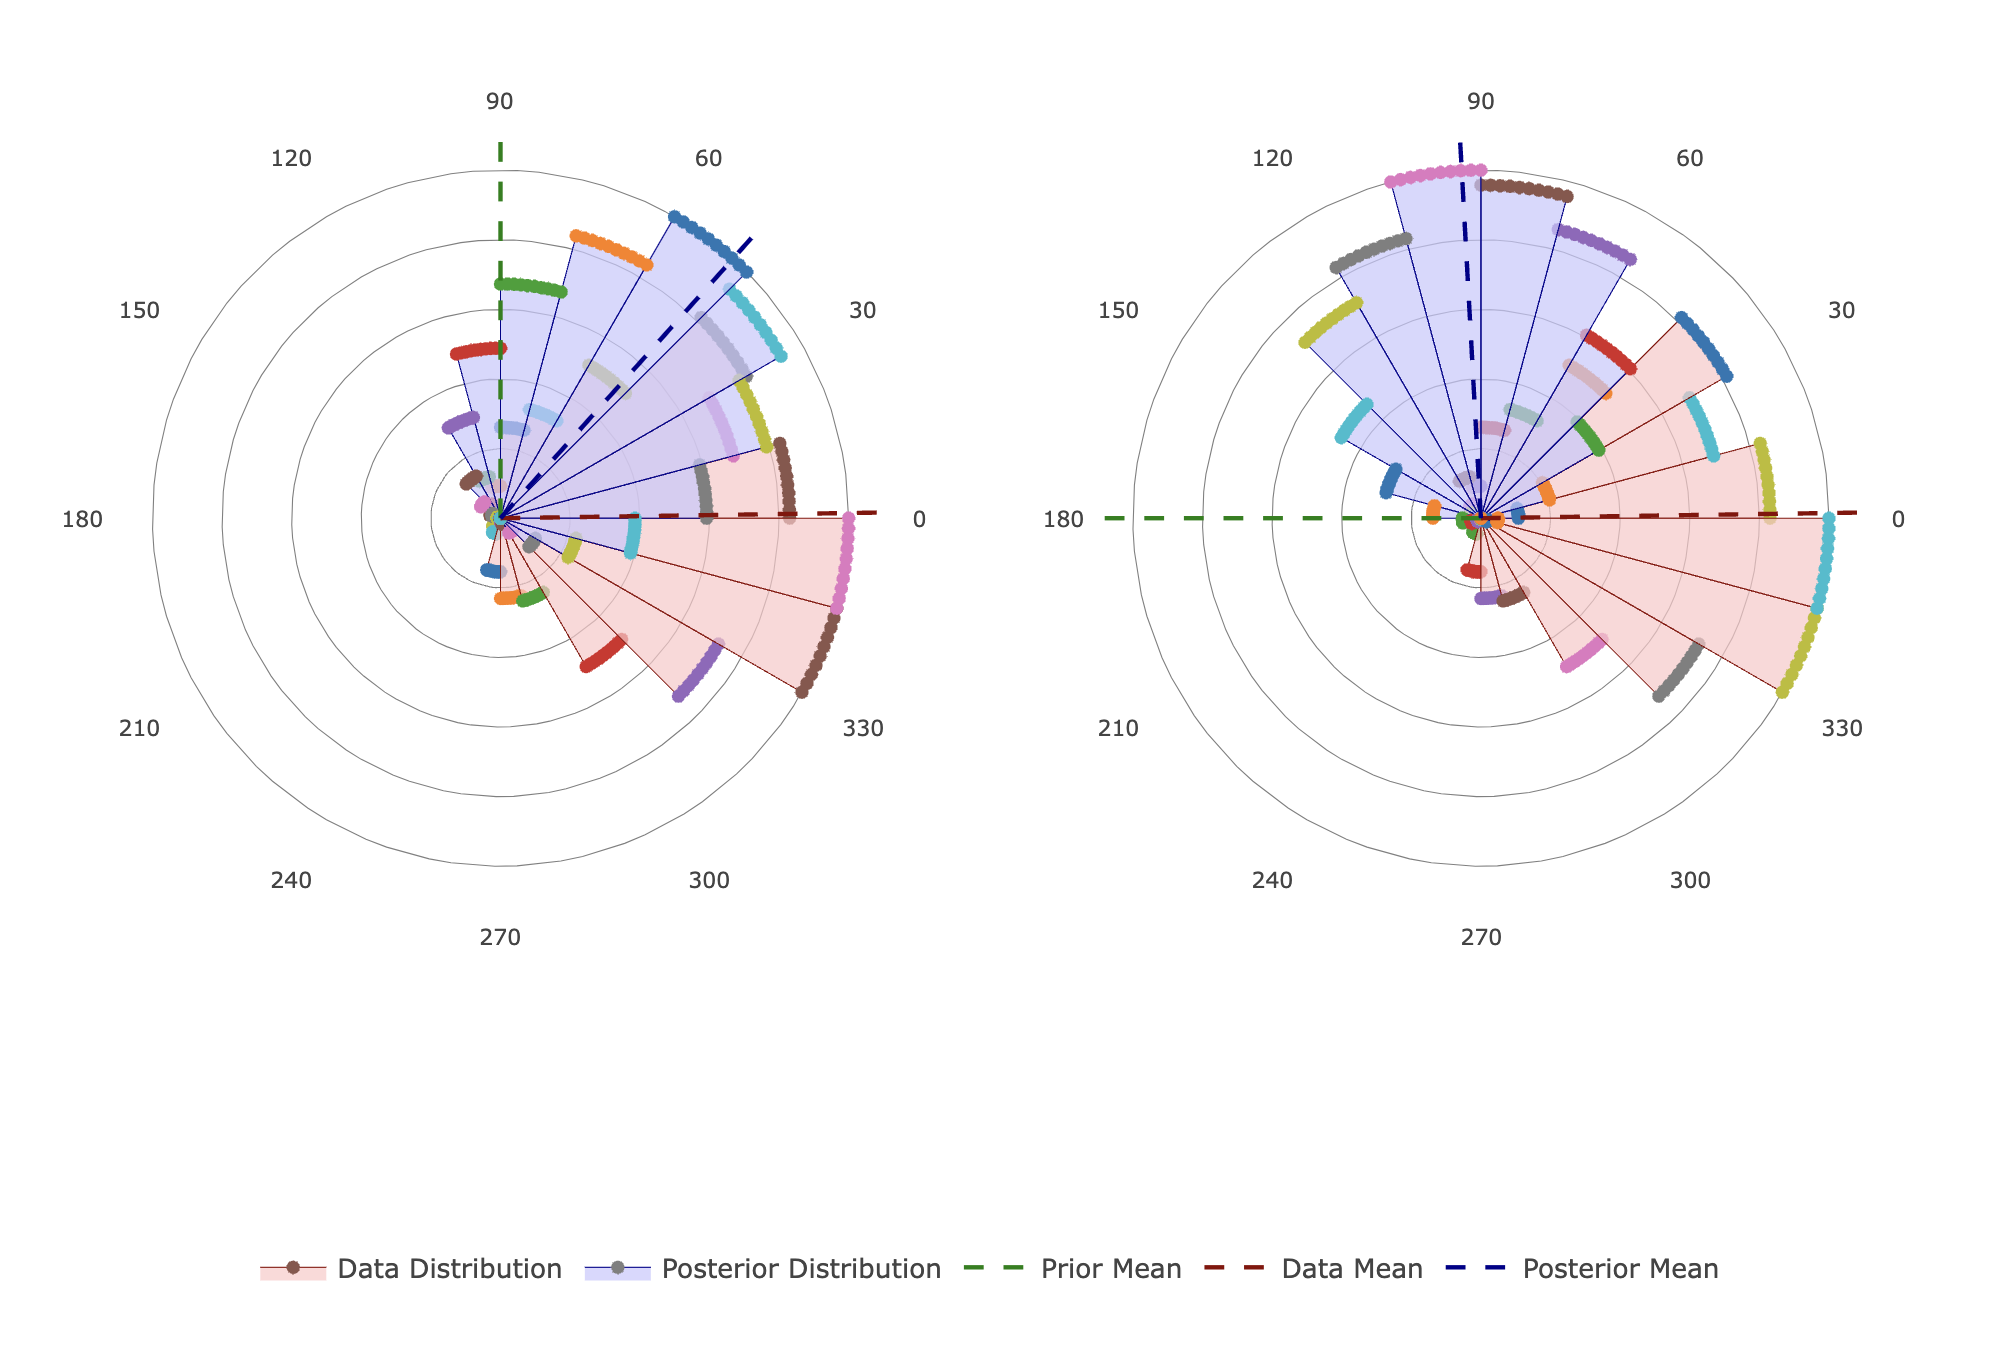
\includegraphics[width=1\textwidth]{../fig/posterior-roseplot.png}
  \end{center}
  \caption{Posterior distribution under prior $\theta_0$: Left $\theta_0 = \pi/2$; Right: $\theta_0 = \pi$}\label{fig:posteriors}
\end{figure}

We can see that the posterior mean is essentially the average of the prior and data means. This is because our manifold is a sphere with equivalent curvature at every point. For manifolds with heterogeneous curvature, we would see less reprojection with respect to the prior mean when curvature is more extreme.

\begin{figure}
  \begin{center}
    
  \end{center}
  \caption{}\label{fig:}
\end{figure}







\section{An Empirical Bayes Extension in the Service of Causality}

Talk about the pre-post treatment idea. What can angles represent? Dont do any code for this, just explain. 

Could a prior on $\kappa$ potentially encode anticipated topological changes?

\section{Limitations and Future Direction}

\newpage

\appendix
\section*{Appendix A.} \label{sc:app_a}
In this appendix we prove the following theorem from
Section \ref{sc:intro}

\newpage 
\bibliography{references}

\end{document}
